\documentclass{article}
\usepackage[utf8]{inputenc}
\usepackage{tikz}
\usetikzlibrary{positioning}
\usetikzlibrary{shapes}

\begin{document}

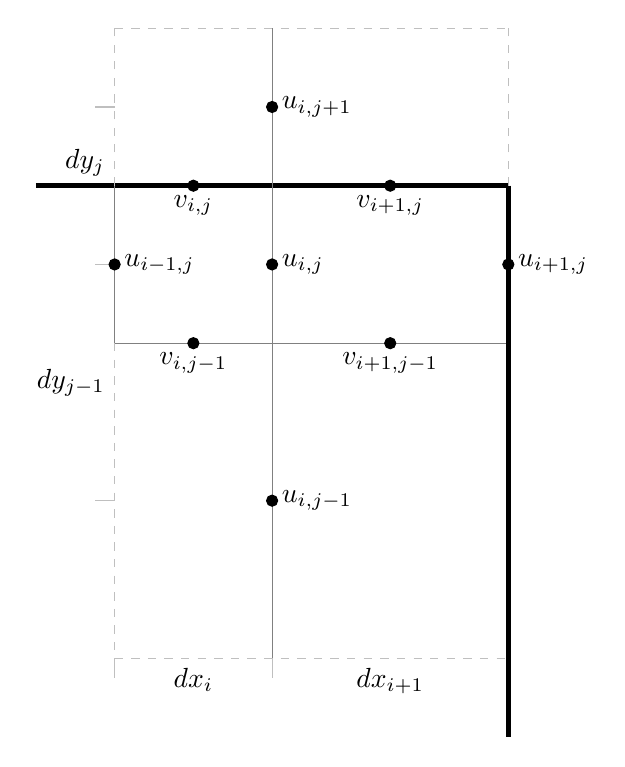
\begin{tikzpicture}
%grid
%horizontal
\draw[black, ultra thick] (-3,1) -- (3,1);
\draw[gray, thin] (-2,-1) -- (3,-1);
%vertical
\draw[gray, thin] (-2,1) -- (-2,-1);
\draw[gray, thin] (0,3) -- (0,-5);
\draw[black, ultra thick] (3,1) -- (3,-6);
%vertical light
\draw[lightgray, thin, dashed] (-2,-1) -- (-2,-5);
\draw[lightgray, thin, dashed] (-2,1) -- (-2,3);
\draw[lightgray, thin, dashed] (3,1) -- (3,3);
%horizontal light
\draw[lightgray, thin, dashed] (-2,3) -- (3,3);
\draw[lightgray, thin, dashed] (-2,-5) -- (3,-5);
%anchor lines
\draw[lightgray, thin] (-2,-5) -- (-2,-5.25);
\draw[lightgray, thin] (0,-5) -- (0,-5.25);
\draw[lightgray, thin] (-2,-3) -- (-2.25,-3);
\draw[lightgray, thin] (-2,0) -- (-2.25,0);
\draw[lightgray, thin] (-2,2) -- (-2.25,2);
%nodes
\filldraw [black] (0,0) circle (2pt) node[anchor=west] {$u_{i,j}$};
\filldraw [black] (0,2) circle (2pt) node[anchor=west] {$u_{i,j+1}$};
\filldraw [black] (3,0) circle (2pt) node[anchor=west] {$u_{i+1,j}$};
\filldraw [black] (0,-3) circle (2pt) node[anchor=west] {$u_{i,j-1}$};
\filldraw [black] (-2,0) circle (2pt) node[anchor=west] {$u_{i-1,j}$};
\filldraw [black] (1.5,1) circle (2pt) node[anchor=north] {$v_{i+1,j}$};
\filldraw [black] (1.5,-1) circle (2pt) node[anchor=north] {$v_{i+1,j-1}$};
\filldraw [black] (-1,-1) circle (2pt) node[anchor=north] {$v_{i,j-1}$};
\filldraw [black] (-1,1) circle (2pt) node[anchor=north] {$v_{i,j}$};
%dx dy anchors
\node[black, thin, anchor=north](dxi) at (-1,-5){$dx_i$};
\node[black, thin, anchor=north](dxip) at (1.5,-5){$dx_{i+1}$};
\node[black, thin, anchor=east](dyjm) at (-2,-1.5){$dy_{j-1}$};
\node[black, thin, anchor=south east](dyj) at (-2,1){$dy_j$};

\end{tikzpicture}
\end{document}
